\chapter{Implementation}
\label{chp:implementation}


% %
% HEADER
% %
The smart elasticity is the ability of a system to dynamically auto-scale resources according to scaling policies determined with machine learning techniques.
%
The smart elasticity service hence provides a resource manager, e.g. a container orchestrator, with the ability to learn the best replication degree for its resources, e.g. deployed containers, with respect to the current cluster state.
%
In this work we propose to implement smart elasticity for Kubernetes leveraging reinforcement learning, that is the most famous technique of unsupervised machine learning.
%
In particular, we focus on $\mathcal{Q}$-Learning, which is the most widely studied reinforcement learning algorithm.
%
In this Chapter we show the adopted reinforcement learning model and how the smart elasticity service has been implemented in the Kubernetes environment.


% %
% Q-LEARNING MODEL
% %
\section{$\mathcal{Q}$-Learning model}
\label{sec:implementation-q-learning-model}

A reinforcement learning algorithm can be used to learn the best scaling policy to adopt in response to cluster state changes without any past knowledge.
%
In this work, we propose an approach that makes use of the $\mathcal{Q}$-Learning algorithm, described in Chapter \ref{chp:reinforcement-learning}.
%
A general $\mathcal{Q}$-Learning algorithm relies on a reinforcement learning model that requires the definition of the parameters:

\begin{itemize}
	
	\item \textbf{State Space} $\mathcal{X}$ where each state $x\in\mathcal{X}$ is a cluster state.
	
	\item \textbf{Action Space} $\mathcal{A}$ where each action $a\in\mathcal{A}$ is a scaling action.
	
	\item \textbf{Quality Function} $\mathcal{Q}:\mathcal{X}\times\mathcal{A}\rightarrow\Re$ where the value $q_{x_{n},a_{n}}=\mathcal{Q}(x_{n},a_{n})$ is the quality of the choice of performing the action $a_{n}$ in the state $x_{n}$ at epoch $n$.
	%
	Notice that, since $\mathcal{Q}$-Learning is an iterative algorithm that updates $\mathcal{Q}$, this function requires an initialization setting $\mathcal{Q}_{0}$.
	
	\item \textbf{Rewarding Function} $\mathcal{R}:\mathcal{X}\rightarrow\Re$ where the value $r_{n}=\mathcal{R}(x_{n})$ is the reward achieved for the state $x_{n}$ at epoch $n$.
	
	\item \textbf{Learning Rate} $\alpha\in (0,1]$ that trades off the importance of sooner versus later quality values. The closer $\alpha$ is to $1$ the more important are future quality evaluations with respect to past ones.
	
	\item \textbf{Discount Factor} $\gamma\in [0,1]$ that trades off the importance of sooner versus later rewards. The closer $\gamma$ is to $1$ the more important are future rewards with respect to past ones. 
	
\end{itemize}

These parameters encapsulate the peculiarities of the domain where the algorithm is applied to and are used by the reinforcement learning agent to determine the optimality of a specific action in a given state, according to the following update:

\begin{equation}
\label{eqn:implementation-q-learning-update}
\mathcal{Q}_{n}(x,a) = 
\begin{cases} 
(1-\alpha_{n})\mathcal{Q}_{n-1}(x,a) + \alpha_{n}(r_{n} + \gamma\max_{b} \mathcal{Q}_{n-1}(x_{n+1},b)) & \text{if } x=x_{n},a=a_{n} \\
\mathcal{Q}_{n-1}(x,a)       & \text{otherwise}           \\
\end{cases}
\end{equation}

In the following, we show and motivate our choice for the aforementioned parameters in the context of smart elasticity.


\subsection{State Space}
\label{sec:smart-elasticity-elasticity-leveraging-q-learning-state-space}
INSERT HERE DESCRIPTION OF THE STATE SPACE (ITERATE WITH PROF).


\subsection{Action Space}
\label{sec:smart-elasticity-elasticity-leveraging-q-learning-action-space}
INSERT HERE THE DESCRIPTION AND MOTIVATIONS OF THE CHOOSEN ACTION SPACE (ITERATE WITH PROF).


\subsection{Quality Function}
\label{sec:smart-elasticity-elasticity-leveraging-q-learning-quality-function}
INSERT HERE THE DESCRIPTION AND MOTIVATIONS OF THE CHOOSEN QUALITY FUNCTION (ITERATE WITH PROF).


\subsection{Rewarding Function}
\label{sec:smart-elasticity-elasticity-leveraging-q-learning-rewarding-function}
INSERT HERE THE DESCRIPTION AND MOTIVATIONS OF THE CHOOSEN REWARDING FUNCTION (ITERATE WITH PROF).


\subsection{Learning Rate}
\label{sec:smart-elasticity-elasticity-leveraging-q-learning-learning-rate}
INSERT HERE THE DESCRIPTION AND MOTIVATIONS OF THE CHOOSEN LEARNING RATE (ITERATE WITH PROF).


\subsection{Discount Factor}
\label{sec:smart-elasticity-elasticity-leveraging-q-learning-discount-factor}
INSERT HERE THE DESCRIPTION AND MOTIVATIONS OF THE CHOOSEN DISCOUNT FACTOR (ITERATE WITH PROF).


% %
% ARCHITECTURE
% %
\section{Architecture}
\label{sec:implementation-architecture}

The smart elasticity service is realized by the Smart Scaler Engine, that is a Kubernetes custom controller implemented as a UAS following the micro-services design pattern.
%
In Figure \ref{fig:implementation-architecture} we show the high-level architecture for the smart elasticity service, represented as a UML component diagram.

\begin{itemize}
	
	\item \texttt{Heapster}: collects cluster performance metrics focused on CPU, Memory and Network utilization in a per-Node and per-Pod basis. 
	%
	Metrics can be queried via the \texttt{K8S REST} interface, which proxies the \texttt{Metric Server}, that is responsible for gathering metrics from \texttt{Heapster Master}.
	
	\item \texttt{Kubernetes}: responsible for containers orchestration. 
	%
	In particular, it deployes containers in a per-Pod fashion and dynamically scales them in/out accordingly with the scaling actions submitted by the \texttt{Smart Scale Engine}.
	%
	It exposes its functionalities with a REST API served by \texttt{Kubernetes Master}.
	%
	The most important functionalities are 
	(i) listing of Smart Scalers,
	(ii) listing of Deployments,
	(iii) watching for Smart Scalers changes,
	(iv) watching for Deployments changes,
	(v) horizontal scaling of Deployments
	(vi) querying of cluster metrics.
	
	\item \texttt{Smart Scale Engine}: realizes the smart elasticity service. It follows a micro-services architecture, where services are:
	
	\begin{itemize}
		
		\item \texttt{Agents Manager}: responsible for the allocation/deallocation of \texttt{RL Agents} accordingly to \texttt{Smart Scalers} instantiated within \texttt{Kubernetes}.
		
		\item \texttt{RL Agent}: this is a reinforcement learning agent, thus it executes the $\mathcal{Q}$-learning loop to determine the scaling actions. Each agent is uniquely associated to a Deployment. In particular it determines the best scaling action with respect to the current cluster state accordingly to the adopted reinforcement learning technique. It submits scaling action to \texttt{Kubernetes} via its REST interface. When this component is asked to produce a new scaling action, the \texttt{StateManager} collects metrics from the \texttt{ClusterMonitor} and aggregates them into a new \texttt{ClusterState}, representing the current cluster state. The latter are then used by the \texttt{RLAgent} to execute the reinforcement learning algorithm to produce the new \texttt{ScalingAction}. The \texttt{RLAgent} reads/writes all data required by the RL algorithm from/to the \texttt{RL Repo}.
		
		\item \texttt{RL Repo}: a data store responsible for storing data required by \texttt{RLAgent} for the execution of the reinforcement learning algorithm, e.g. parameters and reinforcement learning matrices.
		
		\item \texttt{API Gateway}: a REST API server exposing to the outside the services provided by the overall \texttt{Smart Scaler Engine} infrastructure.
		
	\end{itemize}
	
\end{itemize}

From a technological point of view, the \texttt{ScalerAI} has been implemented as a Spring-based REST service, that is a de-facto standard solution for Java enterprise web applications; while the \texttt{RLRepository} has been implemented as a MongoDB datastore, which is a de-facto standard technology for NoSQL document-based datastore. 

Let us now focus on the main interactions flows that realizes smart elasticity.
%
First, we have the loop executed by \texttt{Agents Manager}, that is made of the following steps:
%
\begin{enumerate}
	\item 
\end{enumerate}
%
In Figure \ref{fig:implementation-agents-manager-loop-sequence-diagram} we show the flow of interactions during the loop executed by \texttt{Agents Manager}, represented as a UML sequence diagram.

Then, we have the loop executed by each \texttt{RL Agent}, that is made of the following steps:
%
\begin{enumerate}
	
	\item the \texttt{Orchestrator} asks \texttt{ScalerAI} to compute a new scaling action. The request is submitted to the \texttt{ScalerAIController}, which is the \texttt{ScalerAI} entry-point.
	
	\item the \texttt{ScalerAIController} retrieves the current cluster state from the \texttt{StateManager}. The custer state encapsulates the cluster performance metrics of interest, gathered from the \texttt{ClusterMonitor}.
	
	\item the \texttt{ScalerAIController} asks the \texttt{RLAgent} to compute a new scaling action with respect to the current cluster state.
	
	\item the \texttt{RLAgent} (i) computes the current state $s\in\mathcal{S}$ and, concurrently, (ii) retrieves reinforcement learning data from the \texttt{RLDataManager}, which collects it from the \texttt{RLRepository}.
	
	\item the \texttt{RLAgent} uses he gathered state and data to compute sequentially (i) the rewarding function, (ii) the quality function and (iii) the action.
	
	\item the \texttt{RLAgent} concurrently (i) saves new function values to the \texttt{RLRepository} via the \texttt{RLRepositoryManager} and (ii) encapsulates the computed action into a new \texttt{ScalingAction} returned to the \texttt{ScalerAIController}.
	
	\item the \texttt{ScalerAIController} returns the new scaling action to the \texttt{Orchestrator}.
	
	\item the \texttt{Orchestrator} apply the scaling action.
	
\end{enumerate}
%
In Figure \ref{fig:implementation-rl-agent-loop-sequence-diagram} we show the flow of interactions during the loop executed by each \texttt{RL Agent}, represented as a UML sequence diagram.

\clearpage
\vfill
\begin{landscape}
	\begin{figure}	
		\label{fig:implementation-architecture}
		\centering
		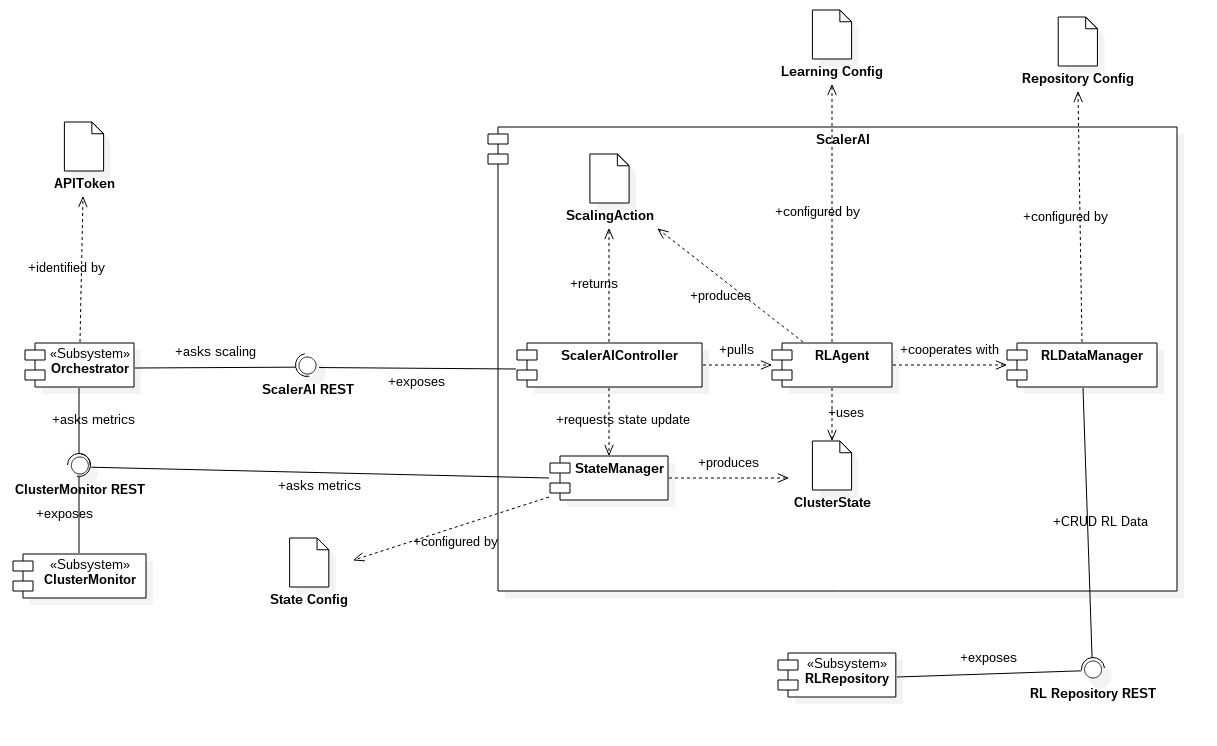
\includegraphics[height=.6\columnwidth, width=.95\columnwidth]{design/implementation-architecture}
		\caption{The architecture of Smart Scale Engine.}
	\end{figure}
\end{landscape}
\vfill
\clearpage
\vfill
\begin{landscape}
	\begin{figure}	
		\label{fig:implementation-agents-manager-loop-sequence-diagram}
		\centering
		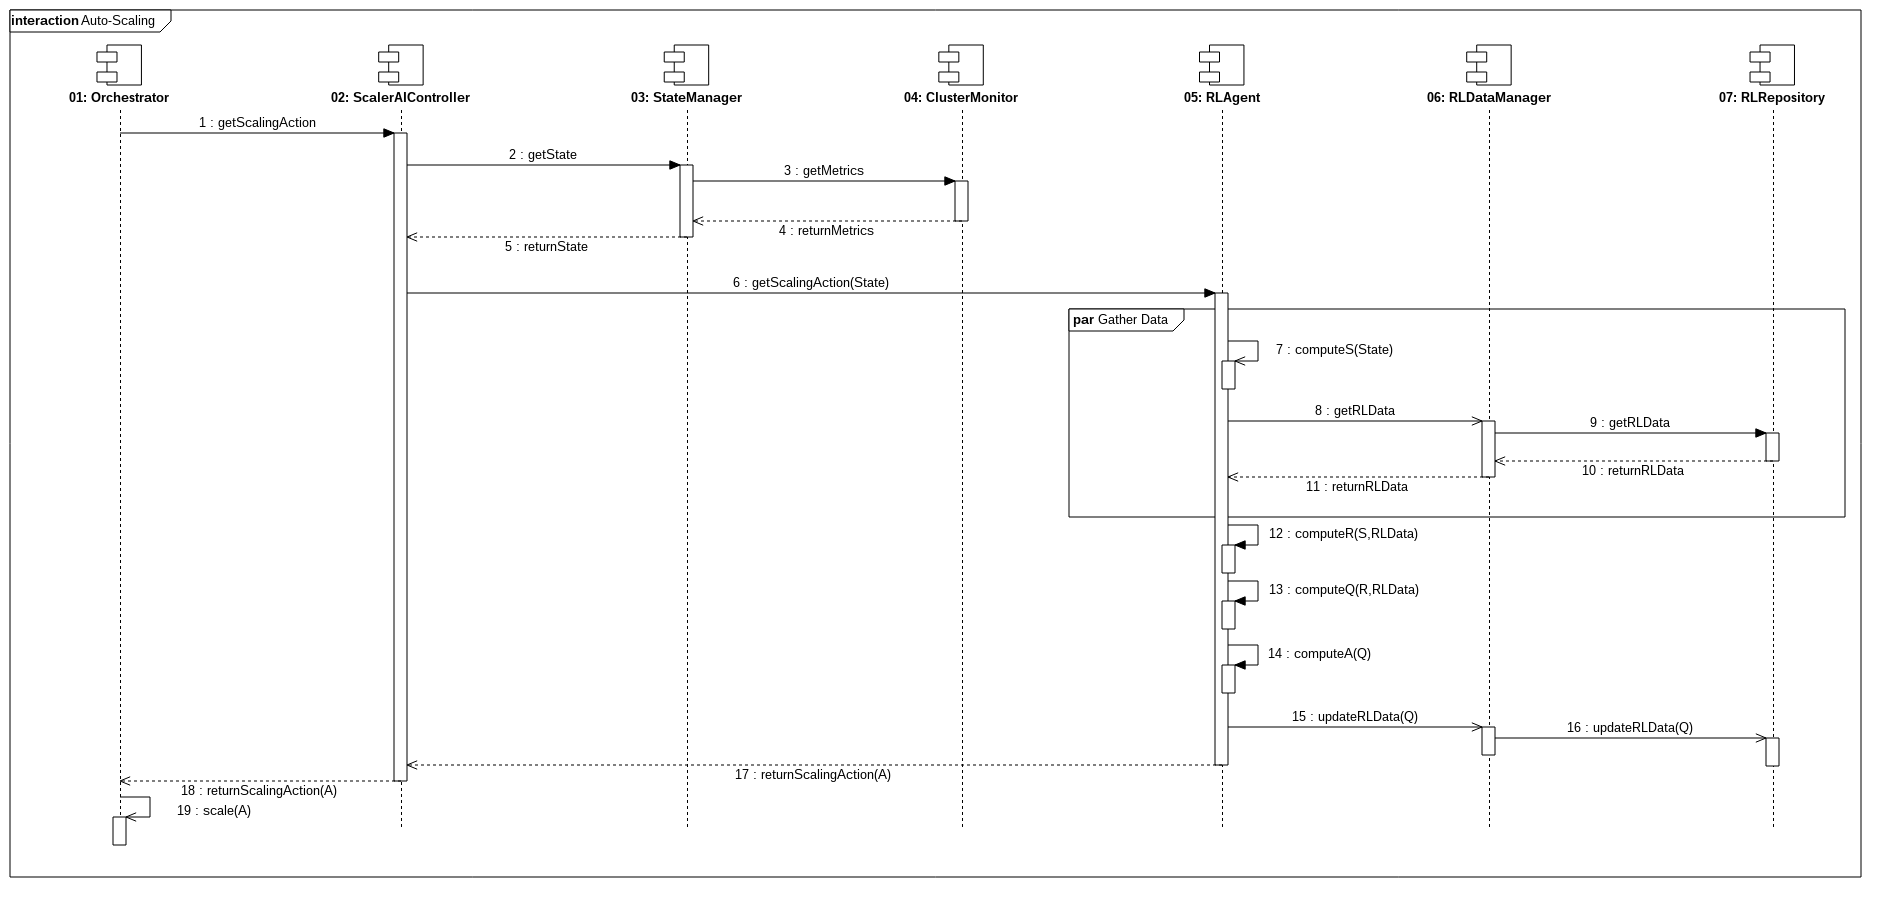
\includegraphics[height=.6\columnwidth, width=.95\columnwidth]{design/implementation-agents-manager-loop-sequence-diagram}
		\caption{The sequence diagram representing the loop executed by the \texttt{AgentsManager}.}
	\end{figure}
\end{landscape}
\vfill
\clearpage
\vfill
\begin{landscape}
	\begin{figure}	
		\label{fig:implementation-rl-agent-loop-sequence-diagram}
		\centering
		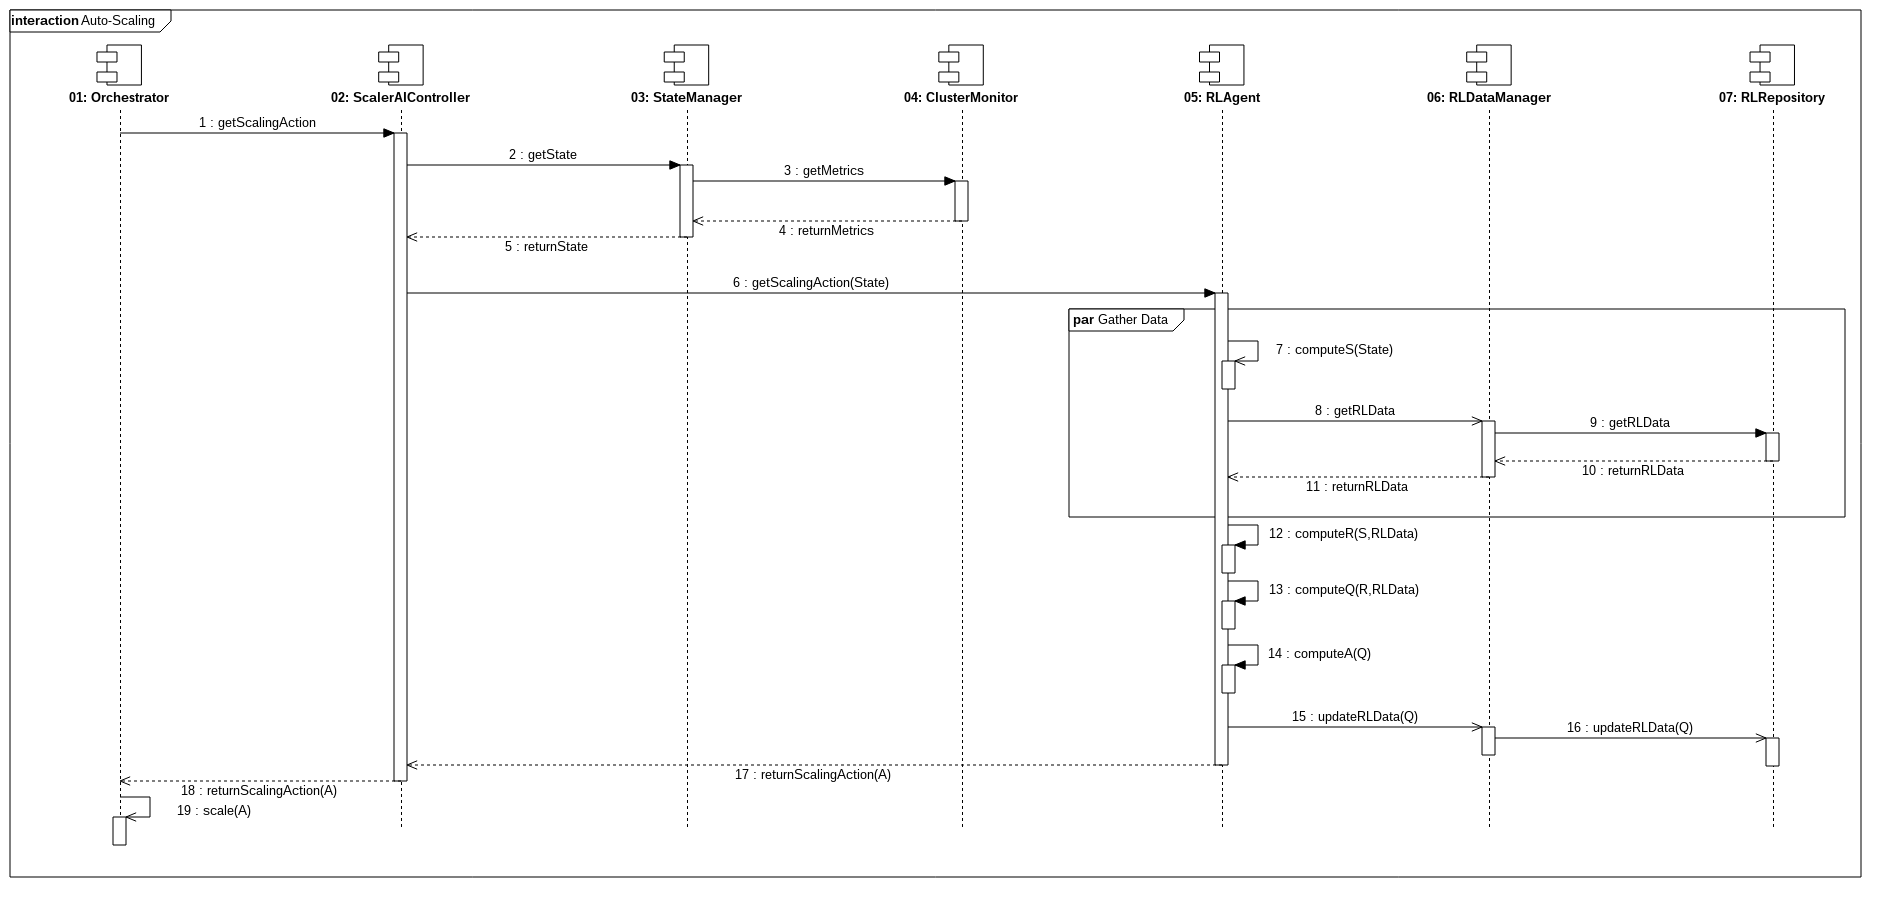
\includegraphics[height=.6\columnwidth, width=.95\columnwidth]{design/implementation-rl-agent-loop-sequence-diagram}
		\caption{The sequence diagram representing the loop executed by a single \texttt{RLAgent}.}
	\end{figure}
\end{landscape}
\vfill
\clearpage


% %
% SMART SCALER
% %
\section{Smart Scaler}
\label{sec:implementation-smart-scaler}
%
A Smart Scaler is a Kubernetes Custom Resource that is associated to an existing Deployment to provide it with smart elasticity.
%
As any other Kubernetes object, a Smart Scaler instance points out a desired system state.
%
In particular, a Smart Scaler instance points out that a given Deployment should be provided with smart elasticity.
%
Smart Scalers are in a $0...1:1$ relation with Deployments, that is each existing Deployment may have zero or one Smart Scaler associated to it.
%
If a Deployment has no Smart Scaler, the smart elasticity service is not provided to it.
%
If a Deployment has a Smart Scaler, the smart elasticity service is provided to it.
%
In particular, since the learning process involved in each Smart Scaler is relative to a any given Deployment, each Deployment should have at most one unique Smart Scaler.

If the Administrator wants to provide an existing Deployment with smart elasticity, it is enough to create a Smart Scaler \textit{MyAppSmartScaler} associated to it.
%
This is the same way the built-in auto-scaling mechanism works, as described in Section \ref{sec:kubernetes-elasticity}.

As Smart Scalers are not built-in objects, a Custom Resource Definition (CRD) should be submitted to Kubernetes to define them as custom objects.
%
%Figure \ref{fig:implementation-smart-scaler-crd} shows the CRD used to define Smart Scalers.
%
The CRD it is pretty self-explanatory.
%
It states that a Smart Scaler is an object provided by the API \textit{gmarciani.com/v1} scoped in namespaces following the common plural, singular and short naming convention.
%
Each Smart Scaler has the following attribute:
%
\begin{itemize}
	
	\item \textbf{deployment:} the name of an existing Deployment to provide with smart elasticity.
	%
	This is a required field.
	
	\item \textbf{algorithm:} the name of the reinforcement learning algorithm to power smart elasticity.
	%
	This is a required field with default value \textit{qlearning}, meaning that $\mathcal{Q}$-learning is the default reinforcement learning algorithm.
	
	\item \textbf{parameters:} a collection of parameters specific to each algorithm. For example, $\mathcal{Q}$-learning requires to specify parameters $rewardFunction$, $\alpha$ and $\gamma$ to customize its behavior.
	
	\item \textbf{replicationMin:} the minimum number of replicas.
	%
	This is an optional field with default value $1$, meaning that at least one replica should be present.
	
	\item \textbf{replicationMax:} the maximum number of replicas.
	%
	This is an optional field, meaning that the replication degree is unbounded.
	 
\end{itemize}
%
Once CRD is submitted, Smart Scalers can be managed as native objects.

For example, to provide an existing Deployment named \textit{MyApp} with a Smart Scaler it is enough to run the command
%
\begin{verbatim}
kubectl create -f MyAppSmartScaler.yaml
\end{verbatim}
%
where \textit{MyAppSmartScaler.yaml} is an instance of a Smart Scaler defined following the schema specified in the Smart Scaler CRD.
%
%\begin{figure}
%	\label{fig:implementation-smart-scaler-crd}
%	\lstinputlisting{code/implementation-smart-scaler-crd.yaml}
%	\caption{Custom Resource Definition for the smart scaler object.}
%\end{figure}

For example, Figure \ref{fig:implementation-smart-scaler-cr} shows a Smart Scaler that realizes smart elasticity for the Deployment named \textit{MyApp} using the Q-learning algorithm with reward function \textit{rfunc1}, alpha equals to 0.7, gamma equals to 0.8 and a replication degree between $1$ and $100$. 
%
\begin{figure}
	\label{fig:implementation-smart-scaler-cr}
	\lstinputlisting{code/implementation-smart-scaler-cr.yaml}
	\caption{A Smart Scaler instance.}
\end{figure}



% %
% REST INTERFACES
% %
\subsection{REST Interfaces}
\label{sec:smart-elasticity-implementation-rest-interfaces}

In this section we detail the REST API exposed by the API Gateway provided by Smart Scaler Engine to manage the learning processes.
%
Furthermore we detail the REST calls executed by Smart Scaler Engine against the Kubernetes Web Server to gather deployment information, performance metrics and to submit scaling actions.

\begin{table}
	\label{tbl:implementation-rest-smart-scaler-engine}
	\centering
	\begin{tabular}{| m{1.5cm} | m{5cm} | m{7.5cm} | }\hline
		
		\textbf{Met.} & \textbf{Resource} & \textbf{Description} \\\hline

		\texttt{GET}	& /status         & Retrieves the status of the overall Smart Scale Engine service \\\hline
		
	\end{tabular}
	\caption{The REST interface exposed by Smart Scaler Engine's Web Server. Each resource path shown here is relative to the server root.}
\end{table}

\begin{table}
	\label{tbl:implementation-rest-kubernetes}
	\centering
	\begin{tabular}{| m{1.5cm} | m{5cm} | m{7.5cm} | }\hline
		
		\textbf{Met.} & \textbf{Resource} & \textbf{Description} \\\hline
		
		\multicolumn{3}{| c |}{/api/gmarciani.com/v1/namespaces/\{namespace\}/} \\\hline
		
		\texttt{GET}  & /smart-scalers & List all deployed smart scalers \\\hline
		
		\texttt{GET}  & /smart-scalers/\{scaler\} & Describe the specified smart scaler \\\hline
		
		\texttt{PATCH} & /smart-scalers/\{scaler\} & Update the specified smart scaler \\\hline
		
		\texttt{DELETE}  & /smart-scalers/\{scaler\} & Delete the specified smart scaler \\\hline
		
		\multicolumn{3}{| c |}{/apis/metrics/v1alpha1/} \\\hline
		
		\textbf{Met.} & \textbf{Resource} & \textbf{Description} \\\hline
		
		\texttt{GET}  & /nodes            & List all nodes metrics \\\hline
		
		\texttt{GET}  & /nodes/\{node\}   & List metrics for the specified node \\\hline
		
		\multicolumn{3}{| c |}{/apis/metrics/v1alpha1/namespaces/\{namespace\}} \\\hline
		
		\texttt{GET}  & /pods & List metrics for all pods in the specified namespace \\\hline
		
		\texttt{GET}  & /pods/\{pod\} & List metrics for the specified pod \\\hline
		
	\end{tabular}
	\caption{The REST interface of interest exposed by Kubernetes's Web Server to manage Smart Scalers and gather metrics.}
\end{table}